\documentclass{sciposter}
\usepackage{lipsum}
\usepackage{epsfig}
\usepackage{amsmath}
\usepackage{amssymb}
\usepackage{multicol}
\usepackage{graphicx,url,physics}
\usepackage[portuges, english]{babel}   
\usepackage[utf8]{inputenc}
%\usepackage{fancybullets}
\newtheorem{Def}{Definition}

\usepackage{fontspec}   % 必须
\setmainfont{Georgia}   % 正文字体
\setsansfont{Georgia}   % 无衬线(如果你想全用 Georgia)
\setmonofont{Courier New} % 等宽字体,可选

\renewcommand{\familydefault}{\rmdefault} 

%\date is unused by the current \maketitle

\rightlogo[1]{logoEngComp}
\leftlogo[1]{logoCefetCampusPetropolis}
% Exibe os logos (direita e esquerda) 
% Procure usar arquivos png ou jpg, e de preferencia mantenha na mesma pasta do .tex
%%%%%%%%%%%%%%%%%%%%%%%%%%%%%%%%%%%%%%%%%%%%%%%%%%%%%%%%%%%%%%%%%%%%%%%%%%%%%%%%
%%% Begin of Document



\begin{document}
%define conference poster is presented at (appears as footer)

% \conference{{\bf SEPEX 2017}, Semana de Ensino, Pesquisa \& Extensão}

%\LEFTSIDEfootlogo  
% Uncomment to put footer logo on left side, and 
% conference name on right side of footer

% Some examples of caption control (remove % to check result)

%\renewcommand{\algorithmname}{Algoritme} % for Dutch

%\renewcommand{\mastercapstartstyle}[1]{\textit{\textbf{#1}}}
%\renewcommand{\algcapstartstyle}[1]{\textsc{\textbf{#1}}}
%\renewcommand{\algcapbodystyle}{\bfseries}
%\renewcommand{\thealgorithm}{\Roman{algorithm}}

% \maketitle

%%% Begin of Multicols-Enviroment
\begin{multicols}{3}

%%% Abstract

\section{Spectrum}

Y-axis$= E^{2}\frac{\dd{J}}{\dd{E}} $, means per \textbf{area} per \textbf{time} per \textbf{solid angle} per \textbf{energy}.


\section{Solid Angles}
\begin{itemize}
    \item An ``isotropic'' distribution
    \[
        \frac{dN}{d\Omega} = \text{constant}
    \]

    \item 
    \[
        \frac{dN}{\sin \theta \, d\theta \, d\phi} = 1, 
        \quad [\theta = 0, \pi], \; \phi = [0, 2\pi]
    \]

    \item 
    \[
        \frac{dN}{d\theta} 
        = \sin\theta \int d\phi \, 
        \frac{dN}{\sin \theta \, d\theta \, d\phi}
        = 2\pi \sin\theta 
        \quad \text{\color{red}{Not a constant!}}
    \]

    \item 
    \[
        \frac{dN}{dx} 
        = \frac{dN}{d\cos\theta}
        = \int d\phi \, 
        \frac{dN}{\sin \theta \, d\theta \, d\phi}
        = 2\pi, 
        \quad \cos\theta = [-1, 1]
    \]
\end{itemize}

\section{No directionality}

\begin{itemize}
    \item It is good to express in typical values

    \item Lamor Radius (Gyro-radius)
    \[
        r_g = \frac{p_\perp}{|q|B}
    \]

    \item 
    \[
        r_g \simeq 3.3\,\text{m}
        \left( \frac{E}{\text{GeV}} \right)
        \left( \frac{e}{|q|} \right)
        \left( \frac{1\,\text{T}}{B} \right)
    \]

    \item Size of the Galaxy $\sim 10~\text{kpc}$

    \item $\text{pc} \simeq 3\times10^{16}\,\text{m}$ \quad or about $3~\text{lyr}$
\end{itemize}

\section{CR Composition}

\begin{itemize}
    \item Right plot shows elemental abundance ratio (normalized at Carbon).
    \item Cosmic ray (CR) composition differs from Solar System abundance.
\end{itemize}

\textbf{Reasons for the difference:}

\begin{enumerate}
    \item \textbf{Different origins:}  
    CRs come mainly from supernova remnants and stellar winds, not the same material as the Solar System.

    \item \textbf{Acceleration bias:}  
    Elements with low first ionization potential (e.g. Mg, Si, Fe) or large charge $|Z|$ are more efficiently accelerated $\Rightarrow$ overrepresented in CRs.

    \item \textbf{Propagation effect:}  
    CRs interact with interstellar matter and produce secondary nuclei (Li, Be, B), leading to their high abundance.

    \item \textbf{Conclusion:}  
    CR composition reflects \textit{acceleration and propagation physics}, not direct stellar nucleosynthesis.
\end{enumerate}


%%% Introduction
\section{Cross Section}
One paritcle interaction, 
\begin{itemize}
  \item $\sigma_{AB}n_{B}L \ll 1  $: very likely to pass through(\textbf{optically thin})
  \item $\sigma_{AB}n_{B}L \gg 1:  $ very likely to interact(\textbf{optically thick})
\end{itemize}

Probability:
\begin{align}
    P=1-e^{-n\sigma L} 
\end{align}
where $\tau=n\sigma L$ is called \textbf{Optical Depth}.

Unit: Barn $1 barn = 10^{-28}m^{2}  $.


\section{Lorentz Factor}

(For motion at velocity $v$ along the x-axis)
\begin{align}
    t' &= \gamma \left(t - \frac{vx}{c^2}\right) \\
    x' &= \gamma (x - vt) \\
    E' &= \gamma (E - vp_x) \\
    p_x' &= \gamma \left(p_x - \frac{vE}{c^2}\right) 
\end{align}



\section{Diffusion Model}

Diffusion-loss equation,
\begin{align}
    \frac{\partial n}{\partial t}=\nabla \cdot \left(D \vec{\nabla}n\right)-\frac{\partial}{\partial E}(n\dot{E})+Q
\end{align}
Diffusion-Convection equation,
\begin{align}
    \frac{\partial}{\partial t}n=\nabla \cdot \left(D\vec{\nabla}n-\vec{V}n\right)-\frac{\partial }{\partial E}(n\dot{E})+Q
\end{align}
with momentum loss term $\dot{p}=-\frac{1}{3}(\nabla \cdot V)p$.

Rigity: $R=\frac{p}{q}$. Motivation: Lamor Radius is propotional to the rigity $r_{g}=\frac{p_{\bot } }{q} $.

Number of particles per phase space: $f=\frac{\dd{N}}{\dd[3]{p}\dd[3]{x}}$.

Differential number density of particles, $n=\frac{\dd{N}}{\dd{p}\dd[3]{x}}=4\pi p^{2}f $.

From diffusion-loss equations, we can imply $$D\frac{\partial f}{\partial r}+\frac{V_{p} }{3}\frac{\partial f}{\partial p}=0 \implies \dd{f}(r,p)=0 \implies f(r_{1},p_{1}  )=f(r_{1},p_{1}  )  $$ 
with definition of flux $I=v n/(4 \pi)=vp^{2}f  $, we have relation
\begin{align}
    \frac{I(p)}{v p^{2} }=\frac{I(p_{ILS} ) }{v_{LIS}p_{LIS}^{2}   }
\end{align}
combining with solar modulation potential $\phi$, we have 
\begin{align}
    \frac{I(p)}{v p^{2} }=\frac{I(p+\phi ) }{v_{lis}(p+\phi)^{2}    }
\end{align}

\section{CR Secondaries}
The full propagation euqation,

\begin{align}
    \begin{aligned}
      \frac{\partial \psi(r,p,t)}{\partial t}&=q(r,p,t)+\overset{\text{Diffusion Convection}}{\nabla\cdot (D_{xx}\nabla \psi-V\psi )}\\
      &+\underset{\text{Re-acceleration}}{\frac{\partial  }{\partial p}p^{2}D_{pp}\frac{\partial }{\partial p}\frac{1}{p^{2} }\psi  }-\underset{\text{Continuous Energy Loss}}{\frac{\partial }{\partial p}\left[\dot{p}\psi-\frac{p}{3}(\nabla\cdot V)\psi\right]}\\
      &-\underset{\text{Fragmentation\& Radi. decay Loss}}{\frac{1}{\tau_{f} }\psi-\frac{1}{\tau_{r} }\psi}
    \end{aligned}
\end{align}
For Fragmentation Loss, for the i-th species, it's loss by $\rightarrow$ j-th species 
\begin{align}
    \frac{\partial n_{i} }{\partial t}=-n_{i}(\frac{\rho}{m})_{ism}\sigma_{i\rightarrow j}v   
\end{align}
 For radioactive decay loss,
 \begin{align}
     \frac{\partial n_{i} }{\partial t}=-n_{i}\frac{1}{\tau_{i} }, \tau_{i} \text{\; is the lifetime}  
 \end{align}

For simple case: Leaky box approx, one species dominates the production, $Q=0$. We have relation,
\begin{align}
    \frac{n_{i} }{T_{e} }=-\frac{n_{i} }{T_{f} }-\frac{n_{i} }{T_{dec} }+C_{i} 
\end{align}
where $C_{i} $ is the production of "i" due to other species, then we can get expression of $n_{i} $,
\begin{align}
    n_{i}=\frac{C_{i} }{1/T_{e}+1/T_{f}+1/T_{dec}   } 
\end{align}

\section{Collision}

We can use Lorentz Invariant $s$,
\begin{align}
    s=(p^{\mu}+p^{\nu}  )^{2} 
\end{align}
where $p^{\mu}=(\frac{E}{c},p^{1},p^{2},p^{3}   ) $.

And definition of Differential cross section,
\begin{align}
    \frac{\dd{\sigma_{i\rightarrow j} }}{\dd{T_{i} }}(T_{i},E_{j}  )
\end{align}

Total corss section: 
\begin{align}
    \frac{\dd{P}}{\dd{t}}=n\sigma
\end{align}
and differential cross section,
\begin{align}
    \frac{\dd{P}}{\dd{t}\dd{T}}=n\frac{\dd{\sigma}}{\dd{T}}
\end{align}
thus, using differential cross section, the number of $\bar{p}$ in interaction $p+p\rightarrow \bar{p}+X$ can be expressed by
\begin{align}
    n_{\bar{p}}(T_{\bar{p}} ) =\left(\int_{E_{th} }n_{p}\frac{\dd{\sigma_{pp\rightarrow\bar{p}X} }}{\dd{T_{\bar{p}} }}(E_{p},T_{p}  )\dd{E_{p} }-n_{\bar{p}}\sigma_{\bar{p}\rightarrow X}    \right)\frac{X}{m}
\end{align}



\section{Electron-Matter Interaction}
A particle interacts with stuff lower energy than
itself causes energy loss through following mechanisms. In matter:
\begin{itemize}
    \item Ionization: Kick off electrons from atoms
    \item Bremsstrahlung: curved trajectory emits photon
\end{itemize}
In space:
\begin{itemize}
    \item Inverse-Compton scattering
    \item Synchrotron radiation
\end{itemize}
With electrons/positrons:
\begin{itemize}
    \item Moller/Bhabba scattering: $e^{-} +e^{+}+ $ electron scattering
    \item Positron annihilation: $e^{-}+e^{+}\rightarrow \gamma+\gamma  $
\end{itemize}

\section{Inverse Compton Scattering}
We assume it as the \textbf{Thomson}(elastic) scattering, because photon energy in CR frame $E_{ph} \sim kT \sim 10^{-4}eV $.

In electron rest frame,
\begin{align}
    &\begin{pmatrix}
    E'_{ph} \\
    E'_{ph} 
    \end{pmatrix}=\begin{pmatrix}
    \gamma &\gamma \beta \\
    \gamma \beta &\gamma 
    \end{pmatrix}\begin{pmatrix}
    E_{ph} \\
    E_{ph} 
    \end{pmatrix}\\
    \implies &E'_{ph}=\gamma(1+\beta)E_{ph}\simeq 2\gamma E_{ph}   \\
    \implies&E_{\gamma} \simeq 2 \gamma E'_{\gamma}\simeq 4 \gamma ^{2}E_{ph}    
\end{align}

Due to the same Lorentz transformation, we know the energy loss of Inverse Compton, is 
\begin{align}
    -\frac{\dd{E_{e} }}{\dd{t}}=\frac{\dd{E_{\gamma} }}{\dd{t}}=\frac{\dd{E'_{\gamma} }}{\dd{t}}
\end{align}
Give the expression of power 
\begin{align}
    \frac{\dd{E'_{\gamma} }}{\dd{t}}=\int E'_{\gamma}\frac{c\dd{\sigma}}{\dd{E'_{\gamma} }}\dd{E'_{\gamma} }\dd{n'_{\gamma} }
\end{align}
working in Thomson limit, th edifferential cross section is,
\begin{align}
    \frac{\dd{\sigma}}{\dd{E'_{\gamma} }}=\sigma_{t}(E'_{ph}-E'_{\gamma}  )\implies \frac{\dd{E'_{\gamma} }}{\dd{t'}}=c\sigma_{t}U'_{ph}   
\end{align}
where $U'_{ph} $ is the photon energy density(in ERS).
\begin{align}
    \frac{\dd{E}}{\dd{t}}=\frac{\dd{E'_{\gamma} }}{\dd{t}}
\end{align}

\section{The Standard Model: Secondary Production}
Positrons are believed to be \textbf{secondary particles}. They are produced by the interaction of primary cosmic rays with the interstellar medium (ISM).

\subsection{Hadronic Interaction Chain}
The production mechanism is a multi-step decay process initiated by high-energy proton-proton collisions (Slide 4, 8, 9):
\begin{enumerate}
    \item \textbf{Pion Production:} A high-energy proton (from cosmic rays) collides with a proton in the ISM (interstellar gas).
    $$ p + p \rightarrow \pi^{\pm} + X \quad (\text{where } \pi^0 \text{ also produced)} $$
    
    \item \textbf{Pion Decay:} The charged pions ($\pi^+$ and $\pi^-$) decay into muons ($\mu^+$ and $\mu^-$).
    $$ \pi^+ \rightarrow \mu^+ + \nu_{\mu} $$
    $$ \pi^- \rightarrow \mu^- + \bar{\nu}_{\mu} $$
    
    \item \textbf{Muon Decay:} The muons then decay, producing positrons and electrons.
    $$ \mu^+ \rightarrow e^+ + \nu_e + \bar{\nu}_{\mu} $$
    $$ \mu^- \rightarrow e^- + \bar{\nu}_e + \nu_{\mu} $$
\end{enumerate}

\subsection{Predicted Positron Fraction}
This secondary production model can be calculated. Because the initial protons have a falling energy spectrum, the resulting secondary positrons also have a falling spectrum. This model predicts that the positron fraction should \textbf{decrease} with increasing energy.

\section{The Positron Anomaly}
The central puzzle in this field is the "positron anomaly," which is a major discrepancy between the theoretical prediction and experimental observation.

\subsection{The PAMELA Discovery}
\textbf{PAMELA}  experiment published results showing that the positron fraction does not fall with energy. Instead, it \textbf{begins to rise} at energies above $\sim 10$ GeV. This was a significant anomaly.

\subsection{Confirmation by AMS and Fermi}
This anomalous rising fraction was not an error. It was subsequently confirmed with higher precision by two other major experiments:
\begin{itemize}
    \item \textbf{Fermi-LAT (Large Area Telescope):} Confirmed the rise, even without a magnet, by cleverly using the Earth's magnetic field to separate $e^+$ and $e^-$.
    \item \textbf{AMS-02 (Alpha Magnetic Spectrometer):} Provided the most precise measurement to date, confirming the rise up to hundreds of GeV.
\end{itemize}

\section{Interpretations and New Sources}
The confirmed anomaly means there must be an \textbf{additional source} (or sources) of high-energy positrons that the secondary production model does not account for.

\begin{itemize}
    \item \textbf{Astrophysical Sources:} The leading candidates are nearby \textbf{Pulsar Wind Nebulae (PWNs)} (Slide 17). These are rapidly rotating neutron stars (pulsars) that create a nebula of high-energy electron-positron pairs. These pairs can escape and propagate to Earth, adding to the positron flux.
    \item \textbf{Exotic Sources:} The anomaly also generated excitement for potential exotic sources, such as the annihilation or decay of \textbf{Dark Matter} particles, which could produce $e^+ e^-$ pairs.
\end{itemize}


\section{Gamma Ray}
For detection, at high energy, pair creation dominates the cross section: $\gamma+A \rightarrow A+e^{+}+e^{-}  $.

For prodection,
\begin{itemize}
    \item Electron $\rightarrow$ matter: Bremsstrahlung gamma rays
    \item Electron $\rightarrow$ radiation: Inverse Compton gamma rays
\end{itemize}

For IC emission,
\begin{align}
    &\frac{\dd{n}}{\dd{E_{\gamma} }\dd{t}}=\int \frac{\dd{n_{e} }}{\dd{E_{e} \dd{\Omega_{e} }}
    }\frac{\dd{N}}{\dd{E_{\gamma} }\dd{t}}\dd{E_{e} }\dd{\Omega_{e} }\\
    &P=E_{\gamma}\frac{\dd{N}}{\dd{E_{\gamma} }\dd{t}} 
\end{align}

PP interactions:

\begin{figure}
    \centering 
    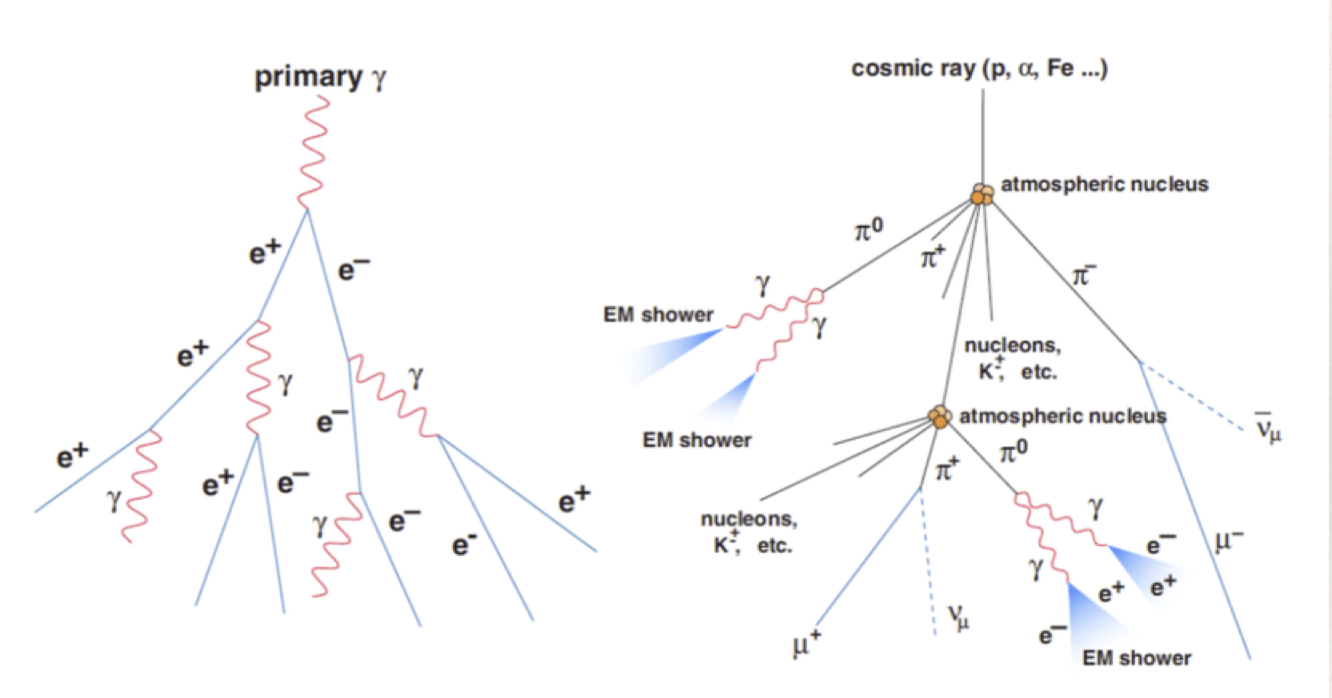
\includegraphics[width=1\textwidth]{1.png}
    \caption{The lightest hadronic states are pions, so they are the primary products from proton-proton interactions}
\end{figure}

\subsection{pionic gamma-ray production}
$pp\rightarrow \pi^{0}\rightarrow \gamma $
Minimum pion energy to produce a photon with energy $E_{\gamma} $ $$E_{min}=E_{\gamma} +\frac{m_{\pi}^{2}  }{4E_{\gamma} }$$ 
Gamma-ray emissivity(photons per volume per time per energy):
\begin{align}
    \frac{\dd{n}}{\dd{E_{\gamma} }}=\iint \frac{\dd{n_{p} }}{\dd{E_{p} }}\frac{\dd{\sigma_{pp \rightarrow \pi} }}{\dd{E_{\pi} }}n_{ISM}c\frac{\dd{N_{\pi \rightarrow \gamma} }}{\dd{E_{\gamma} }}\dd{E_{\pi} }\dd{E_{p} } 
 \end{align}
With angular,
\begin{align}
    \begin{aligned}
        &E_{\gamma}=\frac{m_{\pi} }{2}\gamma (1+\beta \cos \theta') \\
        \implies&\begin{cases}
            \frac{\dd{N}}{\dd{E_{\gamma} }}=\frac{2}{m_{\pi} \gamma \beta},\quad E_{min}(\beta)<E_{\gamma}<E_{max}(\beta)  \\
             \frac{\dd{N}}{\dd{E_{\gamma} }}=\frac{2}{m_{\pi} \gamma \beta}\Theta(E_{\gamma}-E_{min}  )\Theta(E_{max}-E_{\gamma}  )
        \end{cases}
    \end{aligned}
\end{align}


\begin{figure}[ht]
    \centering
    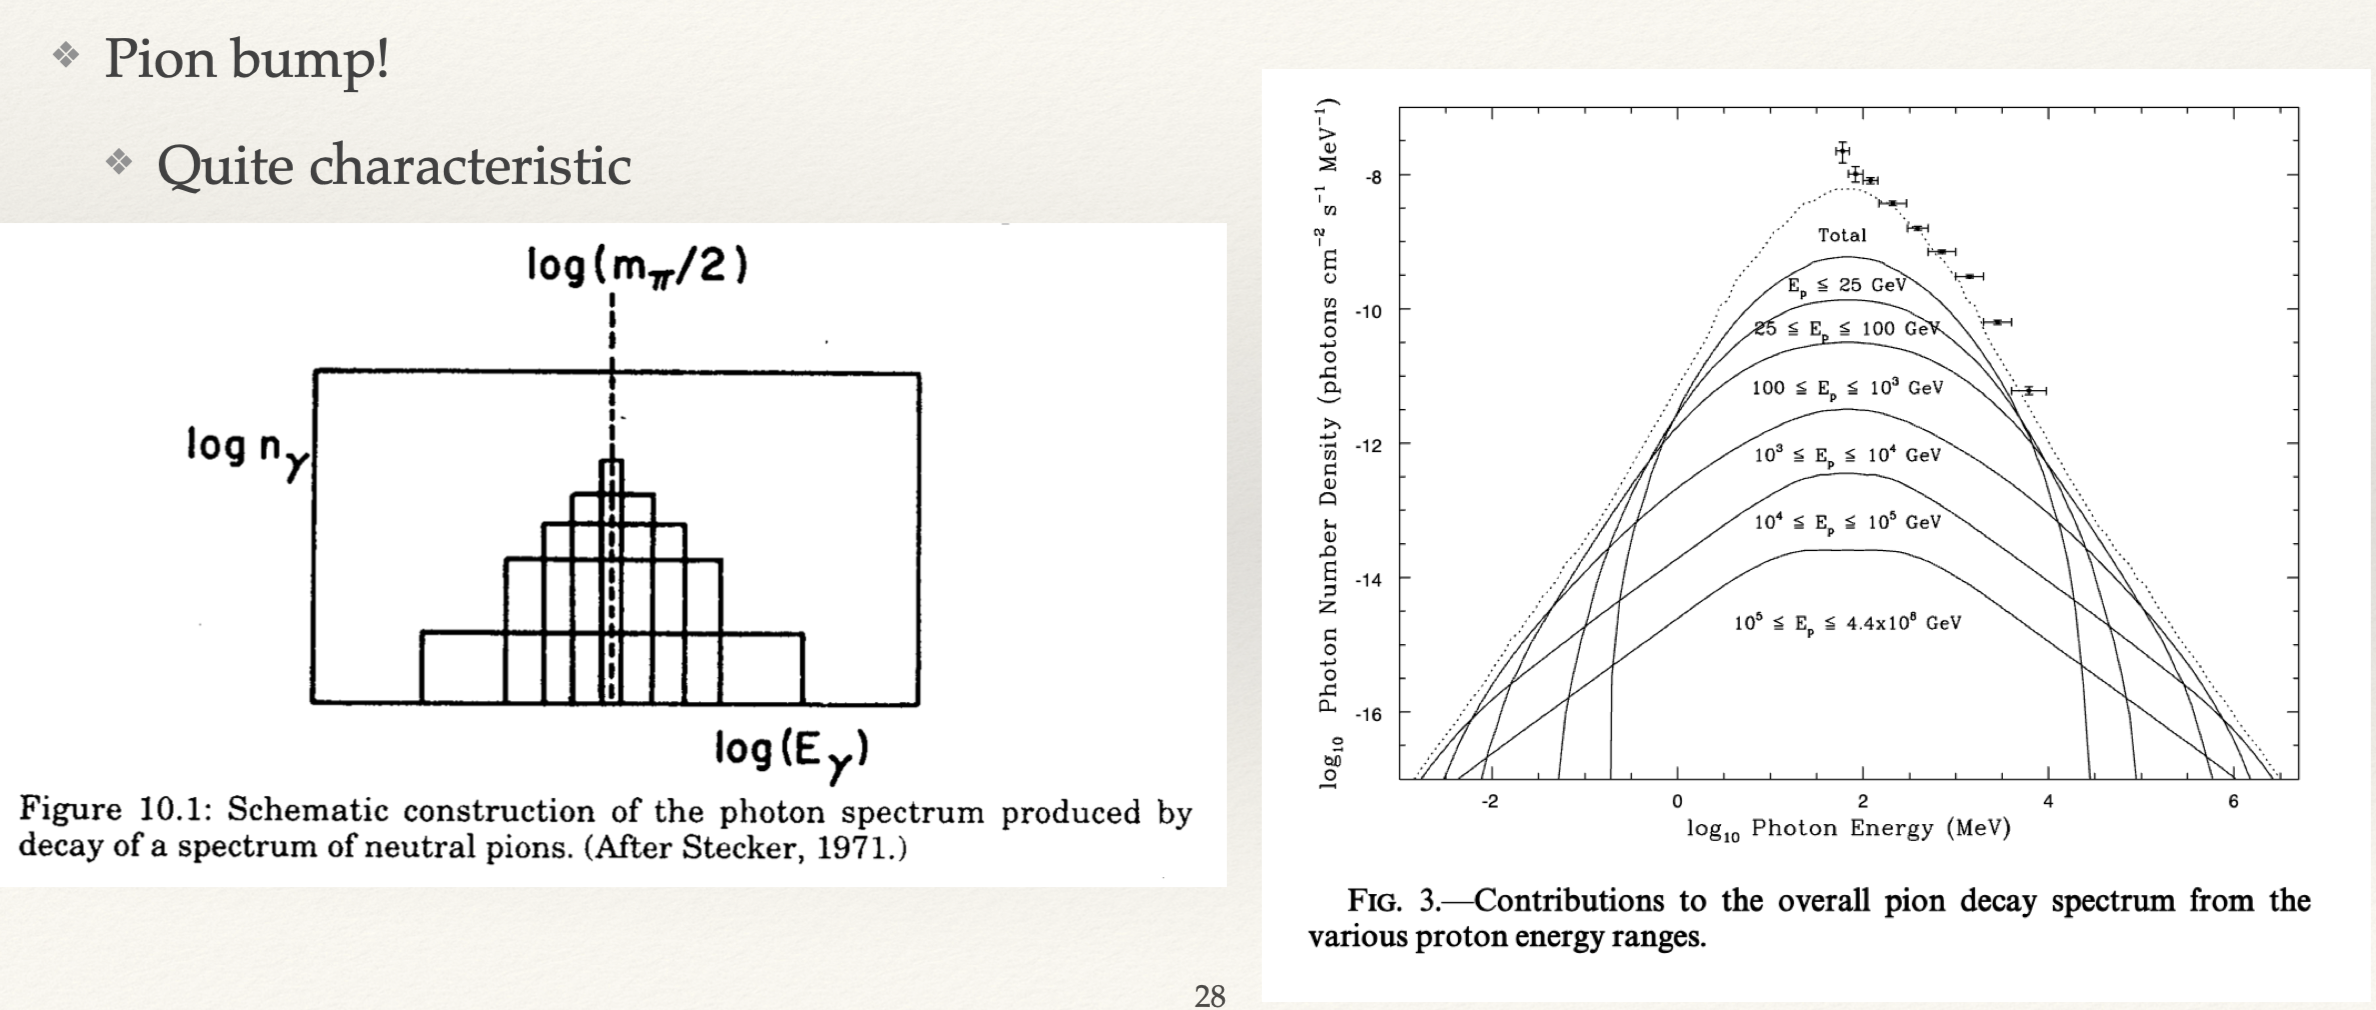
\includegraphics[width= 0.8\textwidth]{2.png}
    \caption{\label{fig:2.png2}
        Shape of pion spectrum
    }
\end{figure}
\section{UHE Cosmic Ray}


\textbf{UHECR Basics}
    \begin{itemize}
        \item \textbf{Definition:} Cosmic rays with energy above the "Knee" ($> 1 \text{ PeV}$).
        \item \textbf{Origin: Extragalactic.}
        \item \textbf{Reason:} The Milky Way's magnetic field is too weak to contain them (based on Larmor Radius calculation).
    \end{itemize}

\textbf{The Four Big Mysteries}
    \begin{itemize}
        \item \textbf{1. Source:} Unknown.
        \item \textbf{2. Direction:} Mostly isotropic (uniform).
            \begin{itemize}
                \item Pierre Auger Observatory found a "hotspot" (anisotropy), but no clear source.
            \end{itemize}
        \item \textbf{3. Composition:} Unknown (Protons? Iron?).
            \begin{itemize}
                \item We measure it from air showers, which depends on interaction models.
                \item \textbf{"Muon Puzzle":} Our models (e.g., QGSJET, SIBYLL) consistently predict fewer muons in the air shower than we actually observe. This implies our models or composition assumptions are wrong.
            \end{itemize}
        \item \textbf{4. Energy Spectrum Features:}
            \begin{itemize}
                \item \textbf{"Ankle":} Point where the spectrum flattens, believed to be the transition from Galactic to Extragalactic cosmic rays.
                \item \textbf{GZK Cutoff:} A sharp drop in particles observed above $\sim 10^{19.5} \text{ eV}$.
            \end{itemize}
    \end{itemize}

 \textbf{The GZK Limit}
    \begin{itemize}
        \item \textbf{Theory:} (Greisen-Zatsepin-Kuzmin) High-energy protons will interact with the Cosmic Microwave Background (CMB) photons ($p + \gamma_{CMB}\rightarrow \Delta^{+}\rightarrow p+\pi^{0} / n+ \pi^{+}   $).
        \item \textbf{Effect:} This interaction causes the proton to lose energy, creating a "horizon." We can only see UHECR sources from relatively nearby ($\sim 100 \text{ Mpc}$) .
        \item \textbf{The Catch:} This cutoff energy only works for protons. If UHECRs are heavy nuclei (like Iron), the cutoff energy is different.
    \end{itemize}

\textbf{Multi-Messenger Solution}
    \begin{itemize}
        \item \textbf{Cosmic Rays:} Are charged, so they are bent by magnetic fields and don't point to their source.
        \item \textbf{Gamma Rays:} Are neutral, but they get absorbed by background light over long distances ($\gamma + \gamma \rightarrow e^+e^-$).
        \item \textbf{Neutrinos:} Are neutral and barely interact. They are the best tool to point directly back to the UHECR sources.
    \end{itemize}




\section{Acceleration}

\subsection*{1. Fermi Acceleration (General Idea)}
\begin{itemize}
    \item After each encounter, particle gains energy:
    \[
        E = \beta^k E_0, \quad N(>E) = N_0 P^k
    \]
    \item Eliminate $k$:
    \[
        N(>E) \propto E^{\frac{\ln P}{\ln \beta}}, \quad 
        \frac{dN}{dE} \propto E^{-1 + \frac{\ln P}{\ln \beta}}
    \]
    \item For first-order Fermi (shock acceleration): 
    \[
        \frac{dN}{dE} \propto E^{-2}
    \]
\end{itemize}

\subsection*{2. Shock Basics}
\begin{itemize}
    \item Upstream: $(\rho_1, v_1, P_1)$, Downstream: $(\rho_2, v_2, P_2)$
    \item Conservation:
    \[
        \rho_1 v_1 = \rho_2 v_2, \quad
        \rho_1 v_1^2 = \rho_2 v_2^2 + P_2, \quad
        \tfrac{1}{2}\rho_1 v_1^3 = \tfrac{1}{2}\rho_2 v_2^3 + \tfrac{3}{2}P_2 v_2
    \]
    \item For strong shocks ($P_1 \simeq 0$):
    \[
        \rho_2 = 4\rho_1, \quad v_1 = 4v_2
    \]
\end{itemize}

\subsection*{3. Particle Acceleration at Shocks}
\begin{itemize}
    \item Relative velocity between up/down stream:
    \[
        V = \frac{3}{4}U
    \]
    \item Energy gain per crossing:
    \[
        \left\langle \frac{\Delta E}{E} \right\rangle = \frac{2}{3}V, 
        \quad \text{Round trip: } \left\langle \frac{\Delta E}{E} \right\rangle = \frac{4}{3}V
    \]
    \item Energy gain factor: $\beta = 1 + \tfrac{4}{3}V$,  
          Escape probability: $P = 1 - U$
    \item For small $U$:
    \[
        \frac{\ln P}{\ln \beta} \simeq -1 \Rightarrow 
        \frac{dN}{dE} \propto E^{-2}
    \]
\end{itemize}

\subsection*{4. Observed Cosmic Ray Spectrum}
\begin{itemize}
    \item Intrinsic (source) index: $\gamma \approx 2.0 - 2.2$
    \item After propagation losses: $\gamma_{\rm obs} \approx 2.7 - 3.3$
\end{itemize}

\subsection*{5. Maximum Energy (Hillas Criterion)}
\begin{itemize}
    \item From Faraday’s law: $\nabla \times \vec{\mathcal{E}} = -\partial_t \vec{B}$
    \item Dimensional estimate:
    \[
        \mathcal{E} \sim BU, \quad E_{\max} = Z e B U L
    \]
    \item Example: young SNR  
    $B \sim 1\,\mu\mathrm{G}$, $U \sim 10^4\,\mathrm{km/s}$, $L \sim 1\,\mathrm{pc}$  
    $\Rightarrow E_{\max} \sim 10^{16}\,\mathrm{eV}$
    \item Hillas plot: $E_{\max} \approx Z B L U$ distinguishes feasible CR sources.
\end{itemize}

\section{Neutrino}


\begin{itemize}
    \item \textbf{History \& Discovery}
    \begin{itemize}
        \item \textbf{Proposal (Pauli, 1930):} Solved the "missing energy" in beta decay ($n \rightarrow p^+ + e^-$). The electron's energy was a continuous spectrum, not a fixed value, implying a third, unseen particle (the neutrino) was present.
        \item \textbf{Discovery (Cowan \& Reines, 1956):} Used a nuclear reactor (a powerful $\bar{\nu}_e$ source) to detect neutrinos via \textbf{Inverse Beta Decay} ($\bar{\nu}_e + p^+ \rightarrow n + e^+$).
    \end{itemize}

    \item \textbf{Weak Interaction \& Parity Violation}
    \begin{itemize}
        \item Neutrinos only interact via the weak force.
        \item \textbf{Wu Experiment (1956):} Observed beta decay from aligned Cobalt-60.
        \item \textbf{Result:} Electrons were emitted asymmetrically (violating Parity/mirror symmetry).
        \item \textbf{Conclusion:} The weak force is "left-handed"---it only interacts with \textbf{left-handed particles} and \textbf{right-handed anti-particles}.
    \end{itemize}

    \item \textbf{The Solar Neutrino Problem}
    \begin{itemize}
        \item \textbf{Experiment (Homestake):} Raymond Davis Jr. used 600 tons of cleaning fluid ($\text{C}_2\text{Cl}_4$) to count solar neutrinos ($\nu_e + {}^{37}\text{Cl} \rightarrow {}^{37}\text{Ar} + e^-$).
        \item \textbf{Problem:} He only detected 1/3 of the neutrinos predicted by the Standard Solar Model.
    \end{itemize}

    \item \textbf{The Solution: Neutrino Mass}
    \begin{itemize}
        \item \textbf{Neutrino Oscillation:} Discovered by Super-Kamiokande (1998) and confirmed by SNO (2001-02). Neutrinos change "flavor" as they travel (e.g., $v_e \rightarrow v_\mu$).
        \item \textbf{Implication:} This oscillation is only possible if neutrinos have **mass**.
        \item \textbf{Significance:} This is physics \textbf{Beyond the Standard Model}, which originally assumed neutrinos were massless.
    \end{itemize}
\end{itemize}

\section{GR\& Cosmos}


\begin{itemize}
    \item \textbf{Principles \& Observations}
    \begin{itemize}
        \item \textbf{Cosmological Principle:} Universe is homogeneous and isotropic on large scales.
        \item \textbf{Hubble's Law:} Galaxies are moving away from us.
        $$v = H_0 d$$
        \item \textbf{Redshift (z):} Caused by the expansion of space (stretching of light).
        $$1+z = \frac{\lambda_o}{\lambda_e} = \frac{1}{a(t)}$$
        where $a(t)$ is the scale factor (with $a=1$ today).
        \item \textbf{CMB (Cosmic Microwave Background):}
        \begin{itemize}
            \item Discovered by Penzias \& Wilson (1960).
            \item Perfect blackbody spectrum with $T = 2.726 \text{ K}$.
            \item Proves the early universe was hot and dense.
        \end{itemize}
    \end{itemize}

    \item \textbf{Friedmann-Lemaître-Robertson-Walker (FLRW) Model}
    \begin{itemize}
        \item \textbf{Einstein's Equation:} Connects spacetime geometry to energy/matter.
        $$G_{\mu\nu} + \Lambda g_{\mu\nu} = \frac{8\pi G}{c^{4}}T_{\mu\nu}$$
        \item \textbf{FLRW Metric:} The metric for a homogeneous, isotropic universe.
        $$ds^{2} = -c^{2}dt^{2} + a(t)^{2}\left[\frac{dr^{2}}{1-kr^{2}} + r^{2}d\Omega^{2}\right]$$
        (Assuming flat, $k=0$, for this course)
    \end{itemize}

    \item \textbf{Cosmic Dynamics (Friedmann Equations)}
    \begin{itemize}
        \item \textbf{1. Friedmann Eq.:} (Hubble parameter $H = \dot{a}/a$)
        $$H^2 = \left(\frac{\dot{a}}{a}\right)^2 = \frac{8\pi G}{3}\rho - \frac{k}{a^2}$$
        \item \textbf{2. Conservation Eq.:} (Fluid equation)
        $$\dot{\rho} = -3H(\rho + P)$$
        \item \textbf{3. Acceleration Eq.:}
        $$\frac{\ddot{a}}{a} = -\frac{4\pi G}{3}(\rho + 3P)$$
    \end{itemize}

    \item \textbf{Cosmic Inventory (Components of the Universe)}
    \begin{itemize}
        \item \textbf{Equation of State:} $P = w\rho$
        \item \textbf{Density Evolution:} $\rho \propto a^{-3(1+w)}$
        \begin{itemize}
            \item \textbf{Matter (Dust):} $w=0 \implies \rho_m \propto a^{-3} \propto (1+z)^3$
            \item \textbf{Radiation:} $w=1/3 \implies \rho_r \propto a^{-4} \propto (1+z)^4$
            \item \textbf{Dark Energy ($\Lambda$):} $w=-1 \implies \rho_\Lambda \propto a^{0} \text{ (constant)}$
        \end{itemize}
        \item \textbf{Critical Density:} $\rho_{cr} = \frac{3H_0^2}{8\pi G}$. $\Omega_i = \rho_i / \rho_{cr}$.
        \item \textbf{Full Friedmann Eq.:}
        $$H(z)^2 = H_0^2 \left[ \Omega_m(1+z)^3 + \Omega_r(1+z)^4 + \Omega_k(1+z)^2 + \Omega_\Lambda \right]$$
    \end{itemize}

    \item \textbf{Cosmological Probes}
    \begin{itemize}
        \item \textbf{Standard Candles (Type Ia Supernovae):} Known luminosity ($L$). We measure flux ($F$) to find Luminosity Distance ($d_L$).
        $$F = \frac{L}{4\pi d_L^2} \quad \text{where} \quad d_L = (1+z) \int_0^z \frac{dz'}{H(z')}$$
        \item \textbf{Key Discovery (1998):} Supernovae were dimmer (farther) than expected. This implies the expansion is \textbf{accelerating}.
        \item \textbf{Deceleration Parameter ($q_0$):} Found to be negative, proving acceleration.
        $$q_0 = \frac{1}{2}\Omega_m + \Omega_r - \Omega_\Lambda \approx \frac{\Omega_m}{2} - \Omega_\Lambda < 0$$
        \item \textbf{Hubble Tension:} $H_0$ measured from the "local" universe (Supernovae) is $\sim 73$. $H_0$ inferred from the "early" universe (CMB) is $\sim 67$. This is a major unsolved problem.
    \end{itemize}
\end{itemize}


\end{multicols}



\end{document}